%%%%%%%%%%%%%%%%%%%%%%%%%%%%%%%%%%%%%%%%%%%%%%%%%%%%%%%%%%%%%%%%%%%%%%%%%%%%%%%%%
% Author: Daniel Keyes
% Type: Master Thesis
% Title: Relocalization for Semi-Dense Visual Odometry
%%%%%%%%%%%%%%%%%%%%%%%%%%%%%%%%%%%%%%%%%%%%%%%%%%%%%%%%%%%%%%%%%%%%%%%%%%%%%%%%%

\documentclass[pdflatex,11pt,a4paper,twoside,titlepage]{scrbook}

%---------packages------------------------------------------------------

\usepackage[english]{babel}
\usepackage[latin1]{inputenc}
\usepackage{a4wide}

%\usepackage{pdfpages}
\usepackage{amsmath}
\usepackage{amsfonts}
\usepackage{amssymb}
\usepackage{mathcomp}
\usepackage{relsize}
\usepackage{mathtools}
\usepackage{algorithm}
\usepackage[noend]{algpseudocode}

\DeclareMathOperator*{\argmin}{arg\,min}

%\addtokomafont{disposition}{\rmfamily}				% uncomment for serif fonts for headings KOMA classes
\usepackage[hang,labelfont=bf]{caption}				% configure captions of images, tables etc.
%\usepackage[footnotesize,sl,SL,hang,tight]{subfigure}		% helpful package for aligning figures next to each other
%\usepackage{captcont}						% continue sufigures over several pages

\usepackage{verbatim}
\usepackage{booktabs}							% publication quality tables for LaTeX
%\usepackage{multirow}						% cells in tables can span multiple rows
%\usepackage{rotating}
\usepackage{fancyhdr}

\usepackage[pdftex]{color,graphicx}
%\usepackage[hang]{caption}
\usepackage{subfig}
\usepackage{color}
\usepackage{float}
\usepackage{hyperref}
\usepackage{fancyref}
\usepackage{listings}
\lstset{keywordstyle=\color{blue}\bfseries\emph, breaklines=true, breakatwhitespace=false}
\lstset{language=C, basicstyle=\footnotesize, commentstyle=\color{green}}
\hypersetup
{
pdftitle = {Relocalization for Semi-Dense Visual Odometry},
pdfauthor = {Daniel Keyes},
colorlinks = {true},
hypertexnames={true},
plainpages={false},
linkcolor={black},
citecolor={black},
filecolor={black},
urlcolor={black},
anchorcolor={black},
menucolor={black},
breaklinks={true}
}

%\setlength{\textwidth}{15cm}
%\setlength{\textheight}{22.0cm}
%\setlength{\oddsidemargin}{0.75cm}
%\setlength{\evensidemargin}{-0.3cm}
%\setlength{\topmargin}{-0.2cm}			% Distance between page top and header
\setlength{\headheight}{15pt}
%\setlength{\parskip}{1.5explus0.5ex}
%\setlength{\parindent}{0pt}				% \noindent
%\renewcommand{\baselinestretch}{1.2}		% Line distance
%\setcounter{secnumdepth}{3}			% Displays Section number down to 3 ranks
%\setcounter{tocdepth}{3}

\newcommand{\clearemptydoublepage}{\newpage{\pagestyle{empty}\cleardoublepage}}
\newcommand{\st}{\stackrel{*}}

%---------document------------------------------------------------------

\begin{document}

\frontmatter

\thispagestyle{empty}
\enlargethispage{2cm} 

\begin{center}
		\vspace*{-3.3cm}
    \rule{\linewidth}{0.5pt} \\
\end{center}


\includegraphics[width=.4\textwidth]{ethlogo}
\vspace{-1.2cm} 

\begin{center}
		\vspace*{0.4cm}
    \rule{\linewidth}{0.5pt} \\
\end{center}


\begin{center}
  \vspace*{.8cm}
  \LARGE \bfseries \boldmath
 Thesis Title
  \vspace*{0.5cm} \unboldmath
\end{center}


\begin{figure}[htb!]
	\centering
  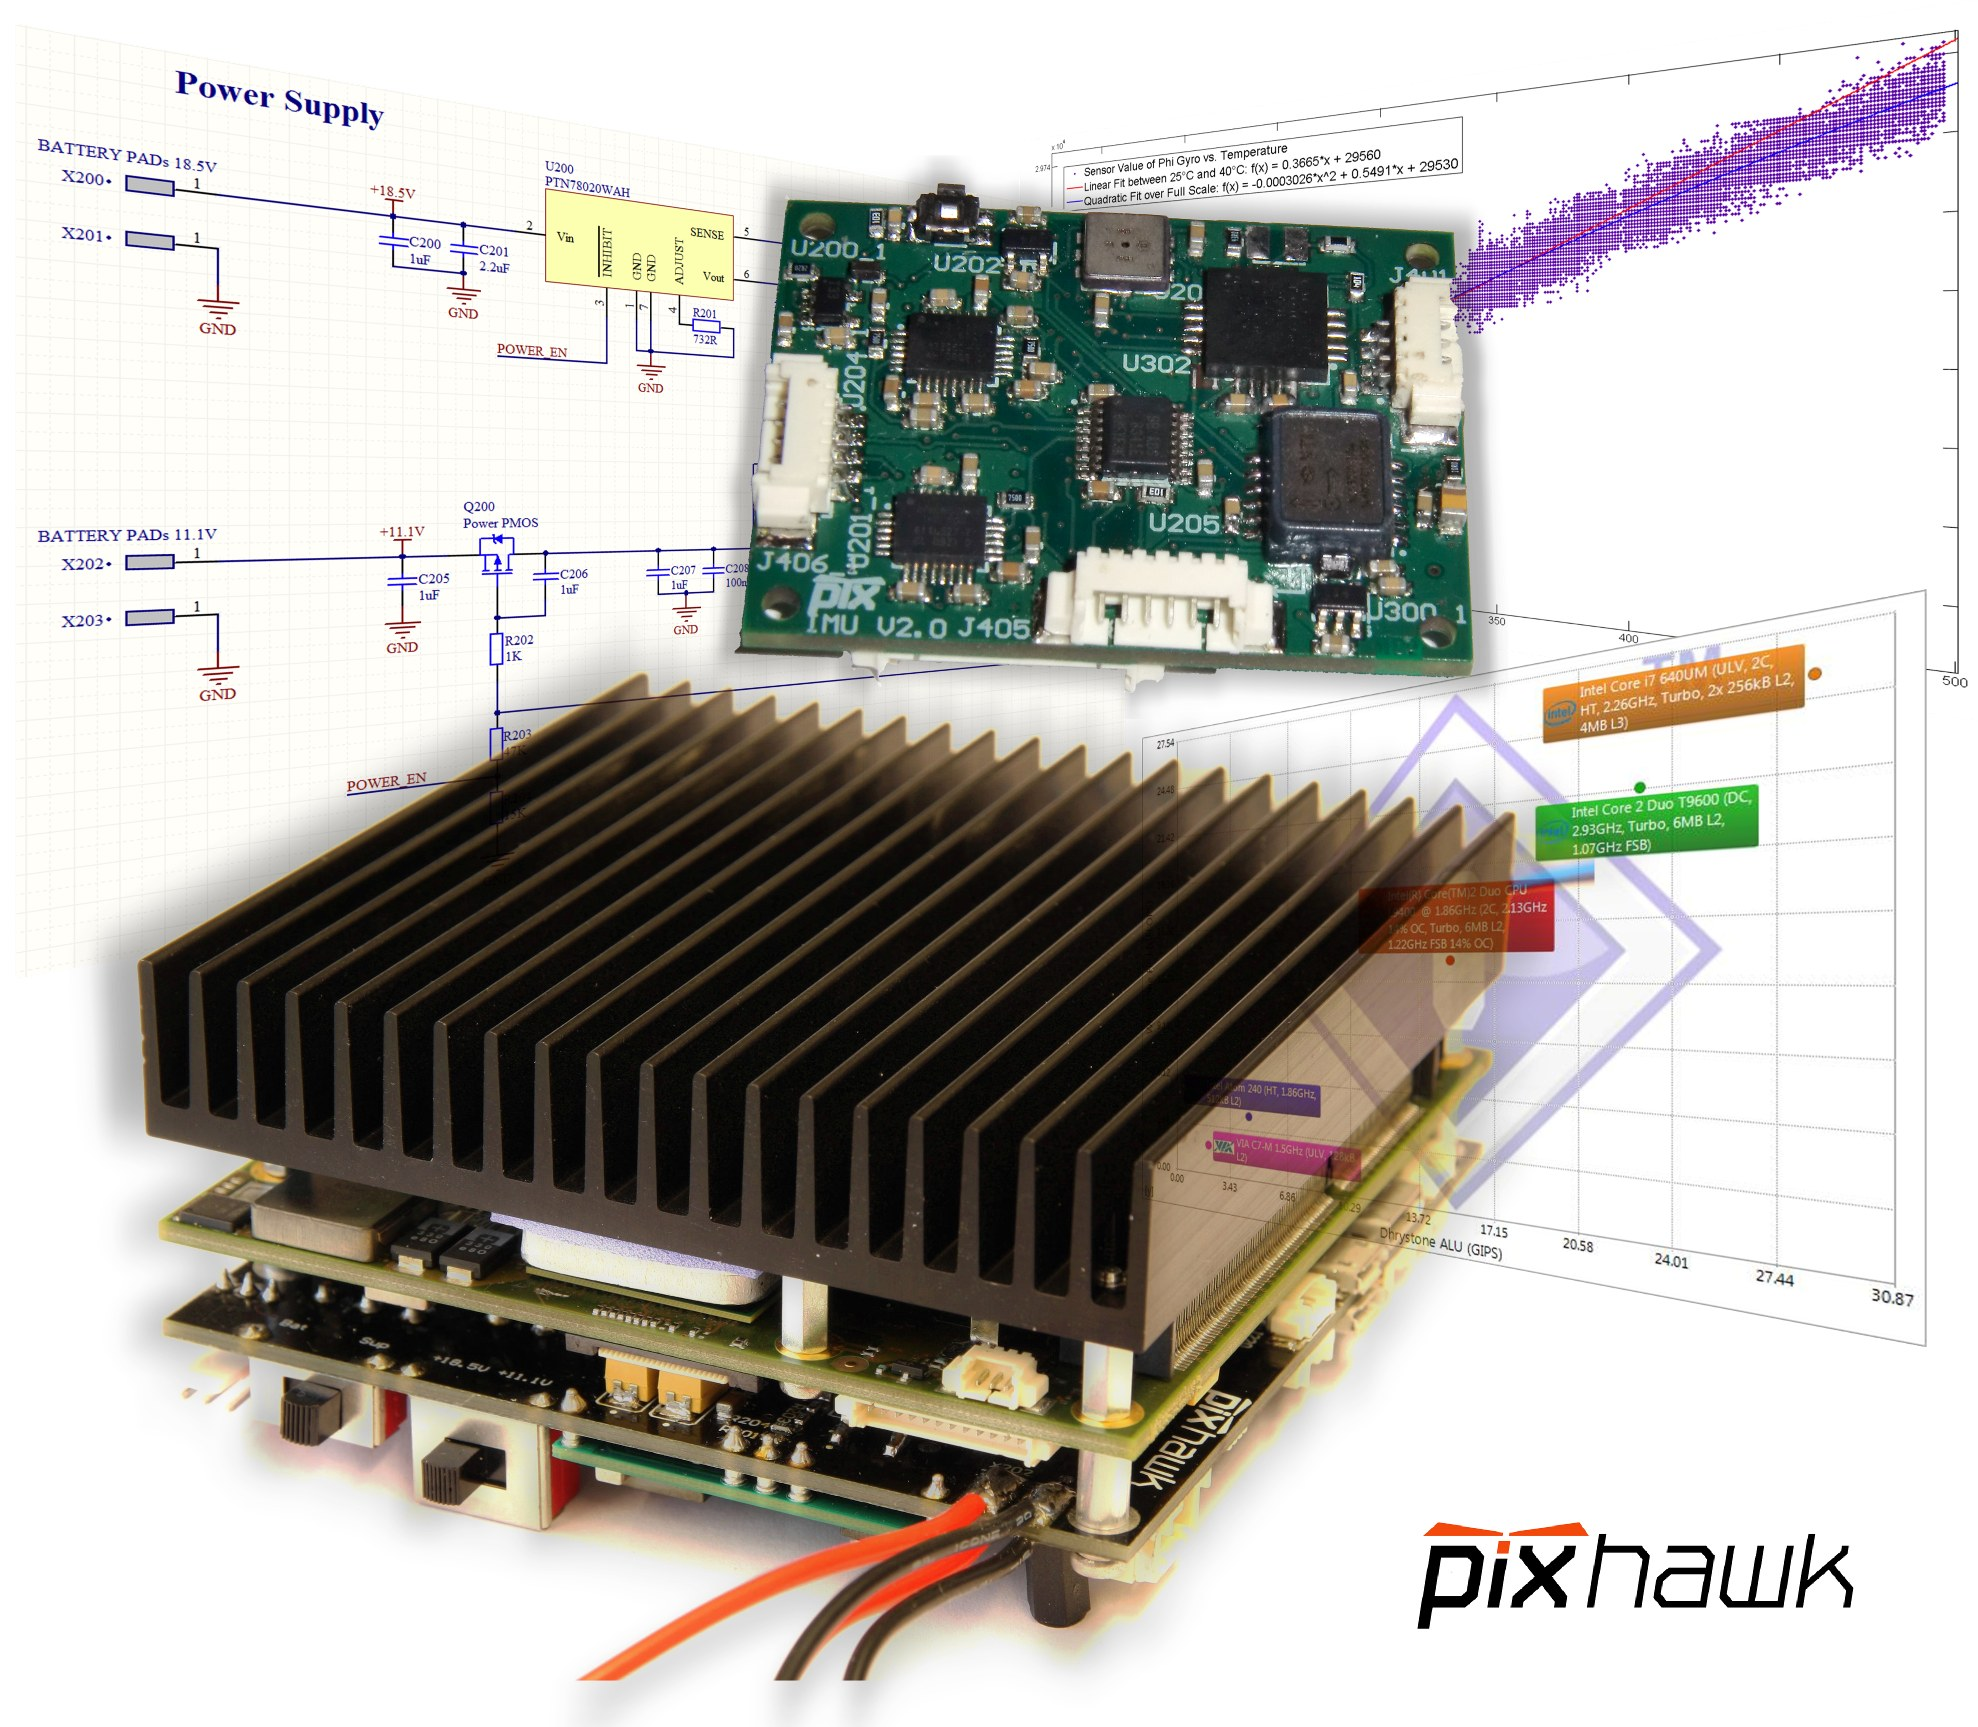
\includegraphics[width=0.9\textwidth]{titlepageimage.jpg}\\
\end{figure}

\begin{center}
  \vspace*{0.5cm}
  \Large
  \textit{Master Thesis CVG Lab\\SS 2017} \\
  \vspace{1cm}
  \Large \mdseries
  Daniel Keyes\\
  \vspace{0.5cm}
\end{center}

\begin{center}
    \rule{\linewidth}{0.5pt} \\
\end{center}

\Large

\begin{tabular}{l@{\hspace{0.5cm}}l}
  Advisors: 	& Federico Camposeco\\
  Professor: 	& Prof. Marc Pollefeys
\end{tabular}

\normalfont \normalsize

\clearemptydoublepage
\chapter{Abstract}

In any camera motion estimation pipeline, the problem of relocalization---determining where a camera is located in a previously constructed map---must be addressed to recover from tracking loss, minimize drift, and remain reliable over time. Whereas traditionally these maps have contained only a very sparse cloud of points, recent developments in visual odometry have shown that it is possible to generate a relatively dense point cloud while tracking camera motion. In this work, we leverage this rich geometric information to perform camera relocalization. We adopt approaches that were previously viable only with dedicated depth-sensing hardware; we analyze our results on two well-known relocalization benchmarks; and we analyze failure cases.

\clearemptydoublepage
\chapter{Acknowledgments}

Acknowledgments to people who supported you. In Semester theses this chapter can be removed.

\clearemptydoublepage

%list of contents, figures and tables
\phantomsection
\addcontentsline{toc}{chapter}{Contents}
\tableofcontents
\cleardoublepage
\phantomsection
\addcontentsline{toc}{chapter}{List of Figures}
\listoffigures
\cleardoublepage
\phantomsection
\addcontentsline{toc}{chapter}{List of Tables}
\listoftables
\cleardoublepage

%customize headers and footers
\pagestyle{fancyplain} % Chapter and Section appear in header
\renewcommand{\chaptermark}[1]{\markboth{#1}{}} % Changes chapter appearence
\renewcommand{\sectionmark}[1]{\markright{\thesection\ #1}} % Changes section appearence
\lhead[\fancyplain{}{\bfseries\thepage}]{\fancyplain{}{\bfseries\rightmark}}
\rhead[\fancyplain{}{\bfseries\leftmark}]{\fancyplain{}{\bfseries\thepage}}
%\cfoot{} % removes page number from footer
\cfoot[\fancyplain{}{}]{\fancyplain{\thepage}{}} %Page number in the first page of a chapter in footer 

%--------- include chapters----------------------------------------------
\mainmatter

\graphicspath{{introduction/}}

\chapter{Introduction}
\label{cha:introduction}

Finding correspondences between recent and formerly visited camera frames is a critical component in many computer vision and robotics systems. For the problem of simultaneous localization and mapping (SLAM), camera relocalization establishes loop closures, which are necessary to correct drift accumulated during the estimate. For applications which do not perform mapping, such as visual odometry (tracking camera movement from video), being able to relocalize is critical to recovering from tracking loss and returning to a known reference frame. This is also relevant to applications on low-power devices, such as mobile robotics or virtual and augmented reality on smartphones, in which it may be desirable to compute a high-quality map ahead of time and track against it later. In some use-cases, such as image retrieval, identifying the pose (i.e.\ the position and orientation) of the viewer in a known map is the goal itself.

In this thesis, we address the problem of relocalization using a recently developed measurement representation called ``semi-dense'' depth maps. In contrast to sparse depth maps, which only store a few nonzero values, and fully dense depth maps, which have a distance stored in every pixel, semi-dense depth maps record the depth of a \textit{significant fraction} of pixels. Recent developments in direct visual odometry \cite{engel2013semi} \cite{engel2017direct} \cite{Forster2014ICRA} have been able to achieve comparable results to depth-based methods, despite only using an RGB camera, and a recurring theme in these methods is the estimation of a semi-dense depth map in each frame. In these works, the maps contain a depth estimate at every pixel with a significant color gradient. This is in contrast to feature-based techniques \cite{klein2007parallel} \cite{murTRO2015}, which only track points located at peaks in the feature response space, and produce a comparatively sparse point cloud. In this thesis, we show how state-of-the-art RGB-D relocalization techniques can be re-applied RGB images paired with semi-dense depth maps.

Monocular (single camera) visual odometry itself comes with a variety of challenges. For example, depth estimation is indeterminate in the case of zero (or very little) camera translation. This can happen if a user rotates a camera around the camera center, perhaps to give a panoramic view of the scene. When camera translation resumes, if no original points are still visible within the viewing frustum, tracking is impossible. Additionally, in lieu of feature matching, direct techniques must make assumptions about camera motion to track pixels from frame to frame. They generally assume small camera movement, and only attempt to track points within a small radius, or (using a motion model) they might search on an epipolar line for the best point correspondence. These assumptions are violated in the case of fast or shaky camera movement, which is common in the real world and further motivates our problem.

Furthermore, these common sources of tracking failure are exacerbated by the scale ambiguity of video from a single camera. In the absence of inertial measurements or calibrated depth cameras, it is impossible to know the true size of observed objects. For example, in a typical structure-from-motion pipeline, the displacement between the initially chosen frames defines the scale. Because of this, multiple independent reconstructions of the same scene may be at arbitrarily different scales. In an on-line system, if tracking fails, we must recover both the original reference frame and the original scale of the scene.

In Chapter 2, we give an overview of related work. Chapter 3 gives a detailed description of the relocalization pipeline. This includes a summary of the visual odometry operation and depth map extraction techniques, as well as an overview of a typical image-based relocalization process. We further expound on techniques for descriptor learning and full \mbox{6-degree-of-freedom} camera localization. Chapter 4 presents concrete results on relocalization benchmarks, and we compare our work to prior visual and depth-based relocalization methods. We conclude in Chapter 5 with a discussion of future work, applications, limitations, and possible extensions to the method.

\cleardoublepage



\chapter{Related Work}



This thesis covers a small portion of the much broader field of camera relocalization. This field addresses a conceptually simple problem: if we have viewed a scene with a camera, and then we return to the same scene later, we would like to figure out where we are. Naturally though, depending on the size and type of the scene, the available sensor hardware, and constraints on performance, accuracy, and runtime, this may require a variety of solutions.

At the highest level, camera relocalization can simply be cast as an image retrieval problem. If we have a database of images labeled with poses, i.e.\ position and rotation, it may be sufficient to simply find a similar image and return that camera's pose. But how do we rate similarity? In their landmark work, Sivic and Zisserman \cite{sivic2003video} answered this by recasting the problem as one of text retrieval, in a so-called ``Video Google'' system. In their work, each image is represented as a set of ``visual words''---which is to say, meaningful predetermined vectors that describe the image. These descriptors are analogous to words in a text document, and as a result, one can compare image similarity using the \textit{term frequency-inverse document frequency} metric commonly used in text search, and the images can be indexed using standard text retrieval techniques. In Sivic and Zisserman's work, they use SIFT descriptors \cite{lowe1999object}, which are desirable due to their invariance to a variety of common camera transforms.

This quantization of images and descriptors into a ``bag of visual words'' has been revisited in many subsequent works. More recently, Philbin \text{et al}.\ \cite{philbin2007object} demonstrate methods to increase the visual vocabulary size to improve the discriminative power of visual words, and they also take into account the original geometric configuration of features with a spatial re-ranking step. Orthogonally, J{\'e}gou \textit{et al}.\ \cite{jegou2008hamming} introduce the use of Hamming embeddings for refining the accuracy of visual words. This is further expounded upon by Arandjelovi\'c and Zisserman \cite{Arandjelovic14a}, and Sattler \textit{et al}.\ \cite{Sattler16CVPR}, who additionally re-rank the top $N$ retrieved results to normalize for common spatial configurations of features.

In addition, J{\'e}gou \textit{et al}.\ \cite{jegou2010aggregating} augment the visual words histogram. They calculate a vector describing the average offset from a visual word center to the actual descriptors present in an image, which they denote the Vector of Locally Aggregated Descriptors (VLAD). Later work \cite{arandjelovic2016netvlad} incorporates this aspect into a deep descriptor learning framework.

In effect, these quantization and index lookup techniques compute a hash of image features that preserves similarity in the descriptor space. There are other ways to compute this as well, for example locality sensitive hashing \cite{datar2004locality}; however, the visual word index approach tends to be dominant due to its small memory footprint compared to other techniques.

Of course, the pose of a database camera is only a rough approximation of the query camera's true pose. If positions of 3D points in the original scene are known, as may be case in a typical structure-from-motion pipeline, we can significantly improve the result by estimating the transform from the retrieved camera to the query camera. This pose registration process is frequently performed in two steps. In the first step, one finds point correspondences between descriptors in both images; in general, this is done by matching descriptor pairs that are nearest neighbors of each other, and may be refined using a ratio test as in \cite{lowe1999object}. This is followed by a model fitting step, in which one finds a relative pose that aligns as many point correspondences as possible. Because many selected points may be outliers, and will not be aligned by the truth model, this is generally performed using a RANSAC loop \cite{fischler1981random}, in which the minimum number of correspondences needed to estimate the pose is repeatedly sampled at random, and the estimated model with the largest consensus set is kept.

This process---image retrieval, point matching, and robust estimation---is sometimes bypassed in favor of direct matching techniques. In this case, all 3D points in the scene are considered as possible matches. This has the potential for increased localization accuracy, since it considers more viable point correspondences. The drawback to this strategy is that it requires a larger memory footprint, since one must perform a search for matching descriptors rather than matching visual vocabulary histograms (which could be easily indexed and stored on disk). In several works \cite{li2010location} \cite{sattler2011fast} \cite{sattler2012image}, proponents explore a prioritized searching scheme to garner an improvement in accuracy while retaining a fast runtime. In this case, the omitted image retrieval step could be seen as a proxy to detect 3D points that ought to be co-visible from a single viewpoint.

Furthermore, these works investigate large-scale urban datasets, which are extremely challenging due to the huge variety of visual imagery. In smaller scenes, such as those investigated by \cite{schmidt2017self}, it may be viable to perform direct matching without any sort of prioritized search.

A variety of newer work eschews the traditional image retrieval process and seeks to provide faster and more task-specific retrieval solutions. Particularly due to the commoditization of depth-sensing cameras (like the Kinect), many works perform relocalization on RGB-D images. Glocker \textit{et al}.\ \cite{glocker2013real} \cite{glocker2015real} relocalize by applying randomized ferns (randomized forests of decision tree stumps) to images to generated encodings, and returning nearest neighbor database images. Shotton \textit{et al}.\ \cite{shotton2013scene} perform regression to directly predict the 3D world coordinate of pixels in a single image using randomized forests, and then perform RANSAC pose estimation on the result. Valentin \textit{et al}.\ \cite{valentin2015exploiting} further improve this by predicting the uncertainty of the random forest regression to refine the final pose estimate. In Schmidt \textit{et al}.\ \cite{schmidt2017self}, the authors learn a dense feature descriptor to use for point correspondence. They leverage prior reconstructions of the scene to automate the task of finding training samples.

Some literature seeks to find descriptors that embody the geometric properties of the scene. These have the advantage of being invariant to changes in lighting conditions and camera viewing angles. For example, Rusu \textit{et al}.\ \cite{rusu2009fast} present a hand-crafted geometric descriptor based on the local normals and curvatures of points in a 3D pointcloud. More recently, Zeng \textit{et al}.\ \cite{zeng20163dmatch} present 3DMatch, which learns a geometric descriptor using a setup similar to \cite{schmidt2017self}.

Still other works seek to use machine learning to replace the pose estimation step. This would be desirable, since RANSAC can be slow in the case of large outlier ratios or high model complexity, and requires some manual tuning. Kendall \textit{et al}.\ \cite{kendall2015posenet} directly regress on the 6-DoF camera pose using a deep neural net, which takes only milliseconds to evaluate. They expand on this idea in later publications \cite{kendall2016modelling} \cite{kendall2017geometric}. In \cite{brachmann2014learning} and \cite{brachmann2016dsac}, the authors learn an alternative point correspondence sampling scheme and hypothesis scoring scheme to replace the methods used in vanilla RANSAC.

In this thesis, we specifically explore the topic of relocalization using semi-dense depth data. In contrast to almost all the previously mentioned work, we assume that a depth camera is unavailable, and that rough, partially empty depth maps have been generated through the use of a purely visual tracking pipeline. Such a method was pioneered by Engel \textit{et al}.\ \cite{engel2013semi}, who proposed it to do visual odometry. In their work, they alternate between depth map propagation and dense tracking using prior depth estimates. Their key insight is that, given an initial depth map and the relative pose to the next frame, they can perform an epipolar line search along each depth ray originating from the first frame to find a likely depth value in the second frame. If we assume that both the inverse depth value from the first frame and the inverse depth value from the second frame are Gaussian-distributed, we can combine the noisy estimates in the manner of an extended Kalman filter.

Engel \textit{et al}.'s work is particularly seminal because it produced high-quality visual odometry by directly minimizing the photometric error between frames, while running as fast as depth-based and feature-based approaches. In a continuation of this work, Engel \textit{et al}.\ published LSD-SLAM \cite{engel2014lsd}, which expresses the frame-to-frame transformations using pose graph in order to perform global bundle adjustment and facilitate large-scale loop closures. Monocular camera odometry drifts in scale over time; therefore, this publication was also notable for the use of similarity constraints (rather than constraints on rigid motion) between poses in the pose graph. To perform large-scale loop closure the authors use OpenFABMAP \cite{glover2012openfabmap}, which is functionally similar to the traditional image retrieval pipelines mentioned earlier. More recently, Engel \textit{et al}.\ released DSO \cite{engel2017direct}, which additionally estimates affine changes in lighting conditions. Another work, SVO \cite{forster2014svo} \cite{forster2017svo} addresses a similar solution.

\cleardoublepage

\chapter{Method Overview}


% TODO: make a figure showing the pipeline as a flowchart

We perform relocalization in several steps. First, to create an initial map of a scene, we perform visual odometry using DSO on each of a set of training videos. For each training sequence, this yields a set of per-frame camera poses and estimated semi-dense point clouds, plus an adjacency list of frames with co-observed points. We then extract features from each keyframe; rather than using an explicit feature detector, we simply evaluate the descriptor at every defined pixel in the semi-dense depth map. In a second pass, we merge multiple keyframe observations of the same point by computing the mean descriptor value, as in [CITE TORSTEN'S PAPER].

In order to perform efficient retrieval of similar images, we compute an inverted index. We cluster features in the training set to create a visual word vocabulary and use the vocabulary to index training keyframes. We use the implementation of [CITE TORSTEN'S PAPER], which additionally filters results by their Hamming embeddings in order to remain descriminative while using a smaller visual vocabulary.

Finally, to relocalize, we compute descriptors for each frame in the test set, again at defined locations in the depth map. Note however that for the test set, we discard the depth information and do not compute the mean descriptor values, so that each test frame can be evaluated independently. Querying the inverted index now returns a list of plausible matches in the training set for each query frame in the test set. We then compute a set of feature correspondences between each training and test frame, which thereby can be used with a RANSAC Perspective-n-Point solver to find the query pose (in the training sequence's frame of reference). We perform geometric verification, i.e.\ compute poses from the top 50 retrieved images, and return the one with the most inlier correspondences.

\section{Visual Odometry}
-run DSO to get map (include algorithm? bookkeeping? note on how things are marginalized?)

\section{Feature Extraction}
In our experiments, we test two kinds of visual features. As a baseline, we use the well-known SIFT feature. We compare this to the learned features of [CITE TANNER'S PAPER], which has demonstrated state-of-the-art performance for use in camera relocalization.

In practice, to extract SIFT features, we first detect a large quantity of SIFT keypoints. Then, for each depth pixel, the closest SIFT keypoint within a small radius ($r=3$ pixels) is assigned. This can be efficiently implemented by, for example, binning features detected in the image into $r \times r$ squares and only checking adjacent bins. After performing this process, some depth pixels may be discarded, e.g.\ if they are not near a peak in the SIFT feature response space, and vice versa.

In contrast to this, it seems reasonable to train a dense descriptor (DEFINE WHAT THAT MEANS), so that we can evaluate it at any point in a semi-dense depth map by simply sampling a pixel of the dense descriptor. TODO: GIVE OVERVIEW OF TANNER'S PAPER

\section{Training a Visual Vocabulary}
	
-for all training images, do clustering
	-approximate clustering
	-assign to clusters

\section{Building the Inverted Index}
-create visual words database
	-description of torsten's stuff? hamming embeddings? inverted index? visual words voting? normalization?


-image matching
	-ratio test. maybe some pseudocode? reference to lowe's paper?
-geometric verification
	-space for PnP derivation? or the definition at least?
-alignment onto original VO and onto GT trajectories
	-sim3 alignment
	-computing relative camera pose, rescaling transformation

\chapter{Experiments}




\chapter{Conclusion}

In this thesis, we have expanded on recent work on semi-dense visual odometry by exploring means of relocalizing a query camera. We applied existing RGB-D techniques using only RGB and our partial depth data. We also investigated the effectiveness of a learned descriptor in this context. Furthermore, we evaluated our pipeline on two public benchmark datasets, and showed that relocalization using a straightforward application of SIFT features is still viable in this domain. Because the topic of direct visual odometry using semi-dense techniques is relatively new, this explores potential opportunities and pitfalls.

\section{Future Work}

We anticipate that many existing techniques can be further explored in the context of semi-dense depth data.

Firstly, many methods \cite{valentin2015exploiting} \cite{schmidt2017self} have made improvements by reckoning about the uncertainty of their estimates. This can frequently be combined with, for example, the Mahalanobis norm in an iterative refinement step to weight observations according to their certainty. In the case of DSO, where we are seeking to minimize the error of Gaussian-distributed observations, the Hessians of our inverse depth estimates give a measure of the uncertainty. For example, in \fref{fig:uncertainty}, we visualize the variance.

\begin{figure}[h]
	\centering
	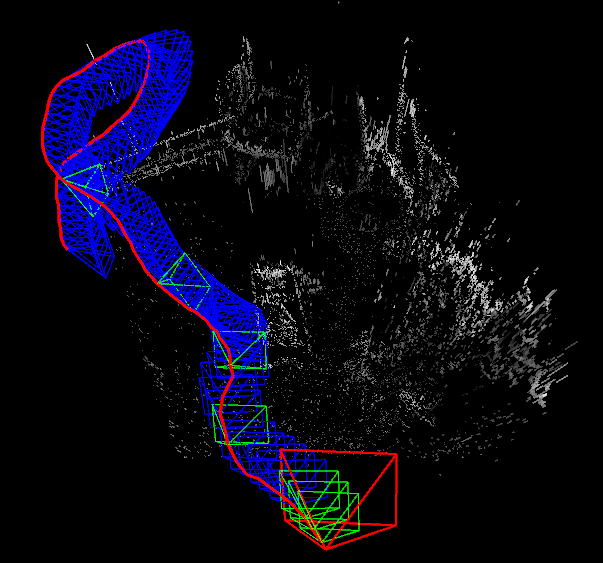
\includegraphics[width=0.4\linewidth]{conclusion/uncertainty.png}
	\caption{DSO at runtime, with only points in the current active window displayed. Active keyframes are marked in green. Here, each point is elongated according to the variance of its inverse depth measurement. As a result, points that are far away or in newly observed areas are stretched out.}
	\label{fig:uncertainty}
\end{figure}

Other approaches also trade accuracy for speed. For example, in small scenes and other scenarios where a camera is likely to revisit the same pose, the randomized ferns approach of \cite{shotton2013scene} would be very effective. These ferns sample random pixels in the RGB-D imagery, so in the case of semi-dense data, one could in-paint the depth or otherwise provide a proxy for the true pixel sample.

Furthermore, since DSO acts on a small window of past keyframes, it would be reasonable to consider windowed temporal data. The authors of VidLoc \cite{clark2017vidloc} do exactly this by training LSTMs on RGB-D video. Additionally, although visual descriptors are generally highly informative, exploring applications of geometric descriptors could be prudent, as in \cite{zeng20163dmatch}, due to the dense, low-drift pointclouds that semi-dense methods generate over time.

For this thesis specifically, we believe that further investigation into failure cases of descriptor matching and pose estimation would be valuable. It also remains to be seen to improve localization for larger scale scenes, and for scenes that are inherently difficult for monocular camera tracking, such as shaky or low frame-rate video. Furthermore, integrating this work directly into a live SLAM pipeline to perform loop closure and recovery from tracking loss would give a complete view of gains that stand to be made.

\cleardoublepage



\backmatter

%Bibliography
%\bibliographystyle{IEEEtran}		% use this for electric engineering thesis (contains support for datasheets)
\bibliographystyle{splncs}		% use this for computer vision thesis
\bibliography{thesis}
\cleardoublepage

%\appendix
%\include{appendix/appendix}

\end{document}
